\chapter{Turvallisuus\label{Turvallisuus}}

Tässä kappaleessa käydään läpi SMS varmenteeseen ja TOTP:hen liittyviä turvallisuusriskejä. 

\section{SMS varmenne}
\begin{figure}[ht]
    \centering
    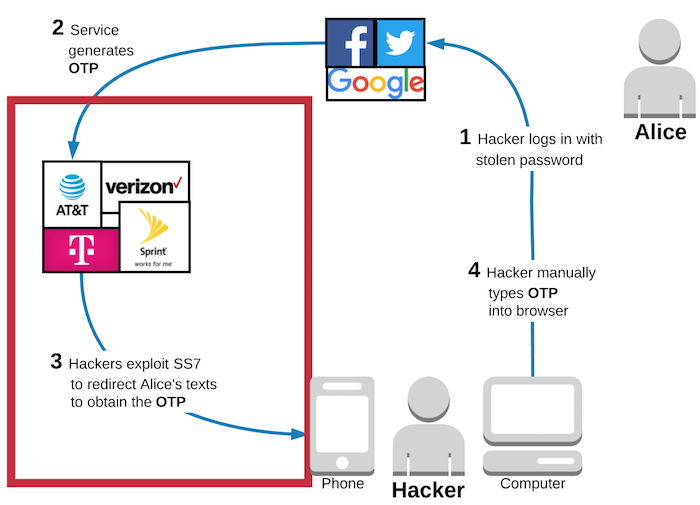
\includegraphics[width=10cm]{template/figures/SS7 attack vulnerable.png}
    \caption{SS7 haavoittuvuus SMS varmentamisessa \citep{2FA_SMS}}
    \label{fig:ss7SMSM}
\end{figure}

SS7 on lyhenne sanoista \emph{Signaling System 7} on vuonna 1975 kehitetty joukko puhelinliikenteen signalointiprotokollille. SS7 protokolaa käytetään puheluiden muodostamiseen, puhelinnumeroiden kääntämiseen ja siirtämiseen, SMS viestien lähettämiseen ja muihin palveluihin. SS7 on vanha systeemi ja siihen liittyy monia havaittuja ja käytettyjä turvallisuusriskejä. Ensimmäinen turvallisuus riski liittyy käyttäjien seuraamiseen. SS7 avulla on mahdollista seurata käyttäjän puhelimen liikkumista missä tahansa maailmaa noin 70 \% tarkkuudella. Toinen turvallisuus riski liittyy puheluiden ja viestien kaappaamiseen. Puheluita ja viestejä on mahdollista siirtää toiseen puhelimeen. Hyökkääjät voivat käyttää näitä menetelmiä hyväkseen. \citep{ss7}

Kuva \ref{fig:ss7SMSM} havainnollistaa kaksivaiheisen kirjautumisen toimintaa, jossa käytetään salasanaa ja tekstiviestillä lähetettävää vahvistuskoodia varmentamiseen. Ensimmäiseksi hyökkääjä kirjautuu varastetuilla tunnuksilla palveluun. Tämän jälkeen palvelu tunnistaa, että käyttäjällä on kaksivaiheinen tunnistautuminen käytössä. Palvelu luo kertakäyttöisen koodin ja lähettää sen tekstiviestinä. Tämän jälkeen siirrytään kuvan \ref{fig:ss7SMSM}  kolmanteen vaiheeseen, joka on merkitty punaisella kehyksellä. Kolmannessa vaiheessa hyökkääjä käyttää SS7 hyökkäystä kertakäyttöisen koodin saamiseksi. Tämän jälkeen hyökkääjä kirjoittaa kertakäyttöisen koodin ja hyökkääjällä on pääsy käyttäjätilille.


\section{TOTP}

Kaksivaiheiseen kirjautumiseen, jossa käytetään TOTP:tä liittyy muutamia turvallisuus Ongelmia.

\begin{figure}[ht]
    \centering
    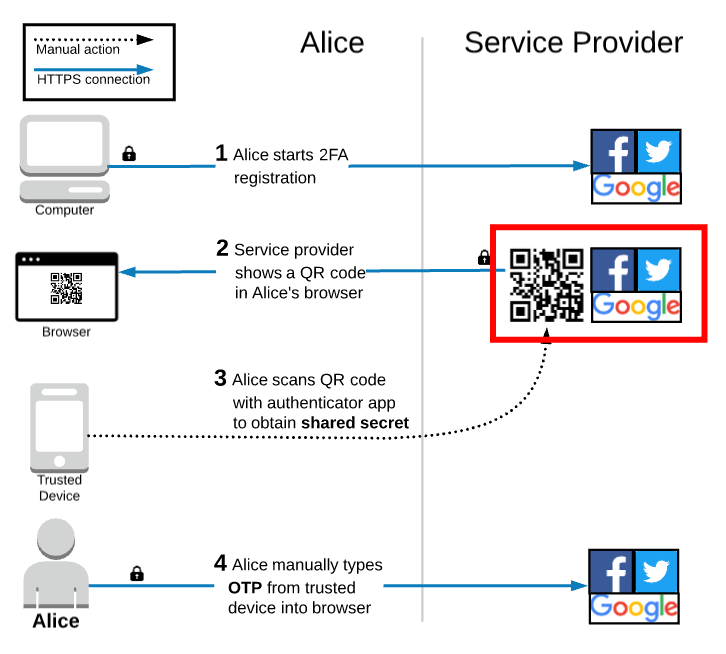
\includegraphics[width=10cm]{template/figures/TOTP service-provider-compromise.png}
    \caption{TOTP salaisen avaimeen liityvä riski \citep{TOTP}}
    \label{fig:TOTP_service_provider}
\end{figure}

Kuvassa \ref{fig:TOTP_service_provider} on merkattu punaisella ensimmäinen TOTP:n käyttämiseen liittyvä turvallisuus ongelma. TOTP:n toiminta perustuu salaiseen avaimeen, jonka palvelun tarjooja antaa käyttäjälle. Salainen avain näytetään yleensä QR koodi muodossa, jonka pystyy skannaamaan puhelimella. Tähän liittyy turvallisuus riski. Jos hyökkääjä saa salaisen avaimen haltuunsa hänellä on pääsy TOTP:n kertakäyttöisiin koodeihin. Näin kaksivaiheisen kirjautumisen hyöty häviää. 

\begin{figure}
    \centering
    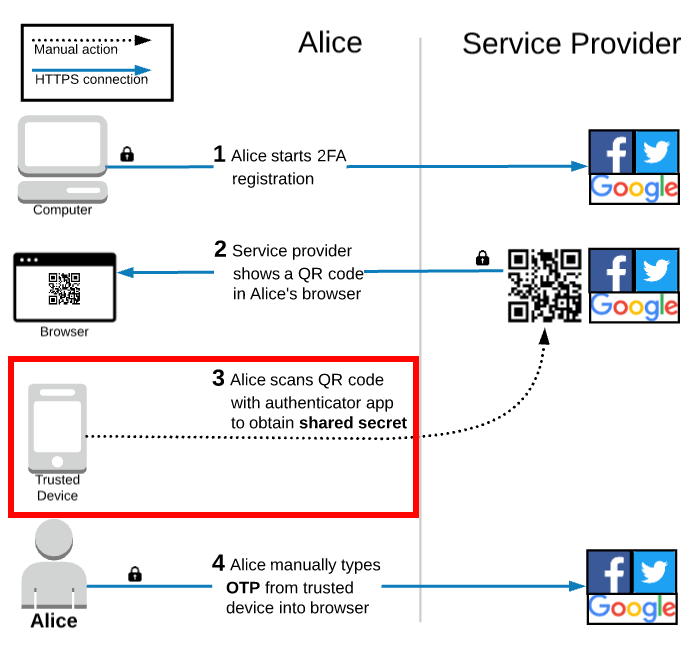
\includegraphics[width=10cm]{template/figures/TOTP trusted-device-compromise.png}
    \caption{TOTP puhelimen turvallisuus riski \citep{TOTP}}
    \label{fig:TOTP_device}
\end{figure}

Kaksivaiheisessa kirjautumisessa missä käytetään TOTP:tä salaisten avaimien tallentamiseen käytetään yleensä puhelinta, joka tässä tapauksessa on luotettu laite. Puhelimeen on tallennettu salaiset avaimet, joiden perusteella OTP koodit luodaan. TOTP:n toinen turvallisuus riski liittyy puhelimeen. Kuvassa \ref{fig:TOTP_device} on punaisella merkitty tätä turvallisuus ongelmaa. Puhelinta pidetään luotettuna laitteena ja oletetaan oikean omistajan olevan vain pääsy siihen. Jos ulkopuolinen varastaa puhelimen ja pääsee käsiksi TOTP koodeihin niin kaksivaiheisen kirjautumisen hyöty häviää.

\begin{figure}[ht]
    \centering
    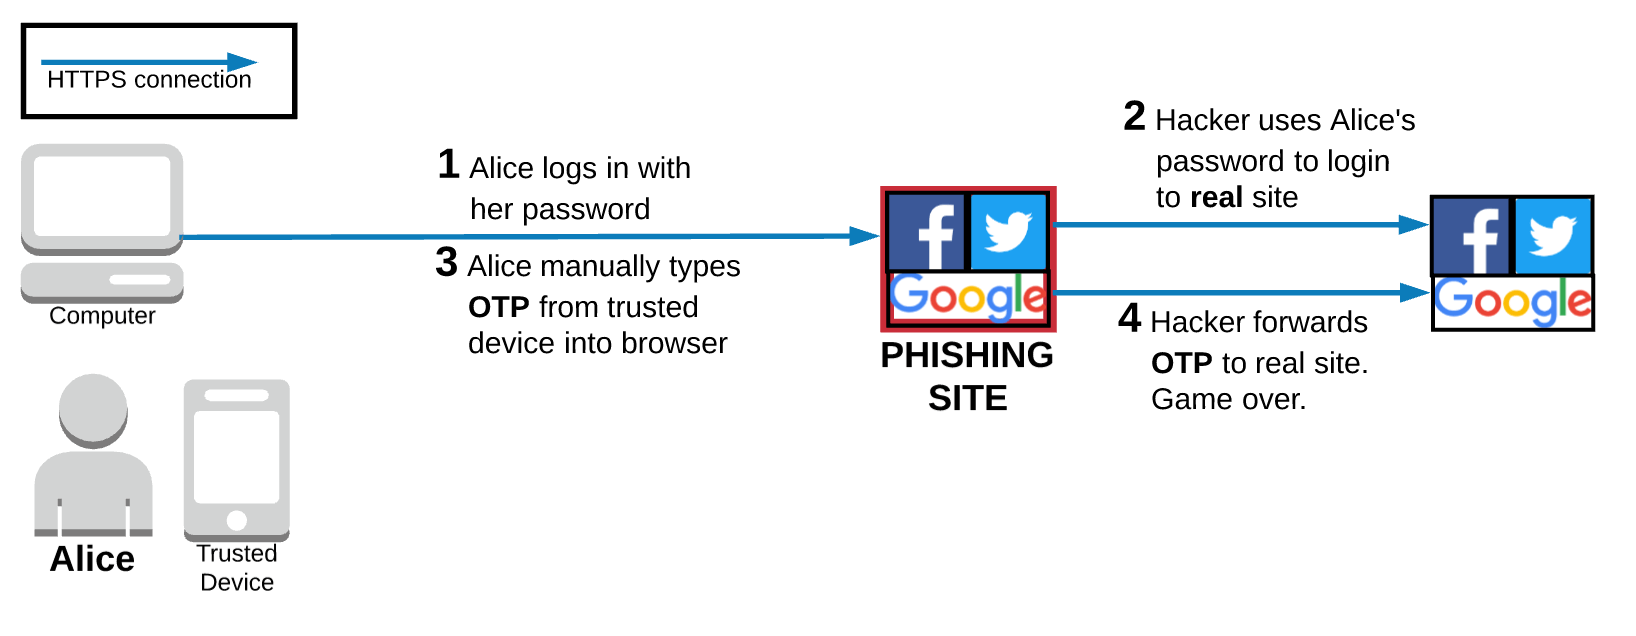
\includegraphics[width=10cm]{template/figures/totp phishing attack.png}
    \caption{TOTP kalastelu sivusto \citep{TOTP}}
    \label{fig:TOTP_phishing}
\end{figure}

Kaksivaiheiseen tunnistautumiseen, jossa käytetään TOPT:tä liittyy myös kalastelun riski. Kalastelu hyökkäyksessä hyökkääjä on tehnyt aidon näköisen verkkosivun, jossa pyydetään käyttäjää antamaan tietoja. Käyttäjä luulee sivuston olevan oikea. Käyttäjä kirjoittaa kirjautumistiedot sekä kertakäyttöisen koodin. Hyökkääjä saa nämä tiedot itselleen ja kirjautuu niiden avulla oikeaan palveluun. Näin hyökkääjä saa pääsyn käyttäjätilille. Kuvassa \ref{fig:TOTP_phishing} on kuvattu kalastelusivun toimintaa. 
 
Kaksivaiheiseen tunnistautumiseen, jossa käytetään TOTP:tä varmentamiseen liittyy turvallisuus riskejä jokaisessa vaiheessa. Turvallisuus ongelmia on salaisten avaimien tallentamisessa palvelun tarjoojalla, puhelin, johon salaiset avaimet on tallennettu sekä kalastelu sivut. 
